\documentclass{article}

\usepackage{tikz}
\usetikzlibrary{intersections}
\usetikzlibrary {calc,through}
\usetikzlibrary {arrows.meta}

\begin{document}

\usetikzlibrary {calc,intersections,through}
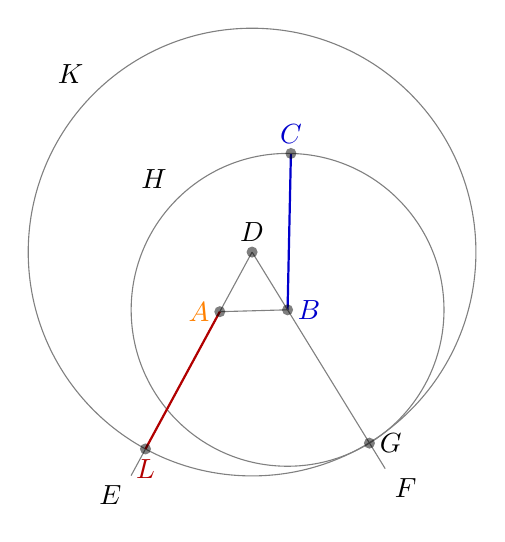
\begin{tikzpicture}[thick,help lines/.style={thin,draw=black!50}]
  \def\A{\textcolor{orange}{$A$}}   \def\B{\textcolor{input}{$B$}}
  \def\C{\textcolor{input}{$C$}}    \def\D{$D$}
  \def\E{$E$}                       \def\F{$F$}
  \def\G{$G$}                       \def\H{$H$}
  \def\K{$K$}                       \def\L{\textcolor{output}{$L$}}

  \colorlet{input}{blue!80!black}    \colorlet{output}{red!70!black}

  \coordinate [label=left:\A]  (A) at ($ (0,0) + .1*(rand,rand) $);
  \coordinate [label=right:\B] (B) at ($ (1,0.2) + .1*(rand,rand) $);
  \coordinate [label=above:\C] (C) at ($ (1,2) + .1*(rand,rand) $);

  \draw [input] (B) -- (C);
  \draw [help lines] (A) -- (B);

  \coordinate [label=above:\D] (D) at ($ (A)!.5!(B) ! {sin(60)*2} ! 90:(B) $);

  \draw [help lines] (D) -- ($ (D)!3.75!(A) $) coordinate [label=-135:\E] (E);
  \draw [help lines] (D) -- ($ (D)!3.75!(B) $) coordinate [label=-45:\F] (F);

  \node (H) at (B) [name path=H,help lines,circle through=(C),draw,label=135:\H] {};
  \path [name path=B--F] (B) -- (F);
  \path [name intersections={of=H and B--F,by={[label=right:\G]G}}];

  \node (K) at (D) [name path=K,help lines,circle through=(G),draw,label=135:\K] {};
  \path [name path=A--E] (A) -- (E);
  \path [name intersections={of=K and A--E,by={[label=below:\L]L}}];

  \draw [output] (A) -- (L);

  \foreach \point in {A,B,C,D,G,L}
    \fill [black,opacity=.5] (\point) circle (2pt);

\end{tikzpicture}

\end{document}
